% -----------------------------------------------------------------
% Document class: Article
\documentclass[ a4paper, twoside, 11pt]{article}
\usepackage{../../macros-general}
\usepackage{../../macros-article}
% Number of the handout, quiz, exam, etc.
\newcommand{\numero}{02}
\setcounter{numero}{\numero}

% -----------------------------------------------------------------
\begin{document}
\allowdisplaybreaks

\begin{center}
\Large Sistemas de Control (EYAG-1005): Lecci\'on \numero \\[1ex]
\small \textbf{Semestre:} 2017-2018 T\'ermino I \qquad
\textbf{Instructor:} Luis I. Reyes Castro
\end{center}
\halfskip

\fbox{

\begin{minipage}[b][\height][t]{\textwidth}
\vspace{0.2 cm}

\begin{center}
\textbf{COMPROMISO DE HONOR}
\end{center}
\vspace{0.4 cm}

\scriptsize
{
Yo, \rule{60mm}{.1pt} al firmar este compromiso, reconozco que la presente evaluaci\'on est\'a dise\~nada para ser resuelta de manera individual, que puedo usar un l\'apiz o pluma y una calculadora cient\'ifica, \linebreak que solo puedo comunicarme con la persona responsable de la recepci\'on de la evaluaci\'on, y que cualquier instrumento de comunicaci\'on que hubiere tra\'ido debo apagarlo. Tambi\'en estoy conciente que no debo consultar libros, notas, \linebreak ni materiales did\'acticos adicionales a los que el instructor entregue durante la evaluaci\'on o autorice a utilizar. Finalmente, me comprometo a desarrollar y presentar mis respuestas de manera clara y ordenada. \\

Firmo al pie del presente compromiso como constancia de haberlo le\'ido y aceptado. 
\vspace{0.4 cm}

Firma: \rule{60mm}{.1pt} \qquad N\'umero de matr\'icula: \rule{40mm}{.1pt} \hspace{0.5cm} \\[-0.8ex]
}

\end{minipage}

}

\vspace{\baselineskip}



% =============================================
\begin{problem}
Considere un sistema cuya respuesta de la frecuencia es como se muestra en la figura de abajo. 

\begin{figure}[htb]
\centering
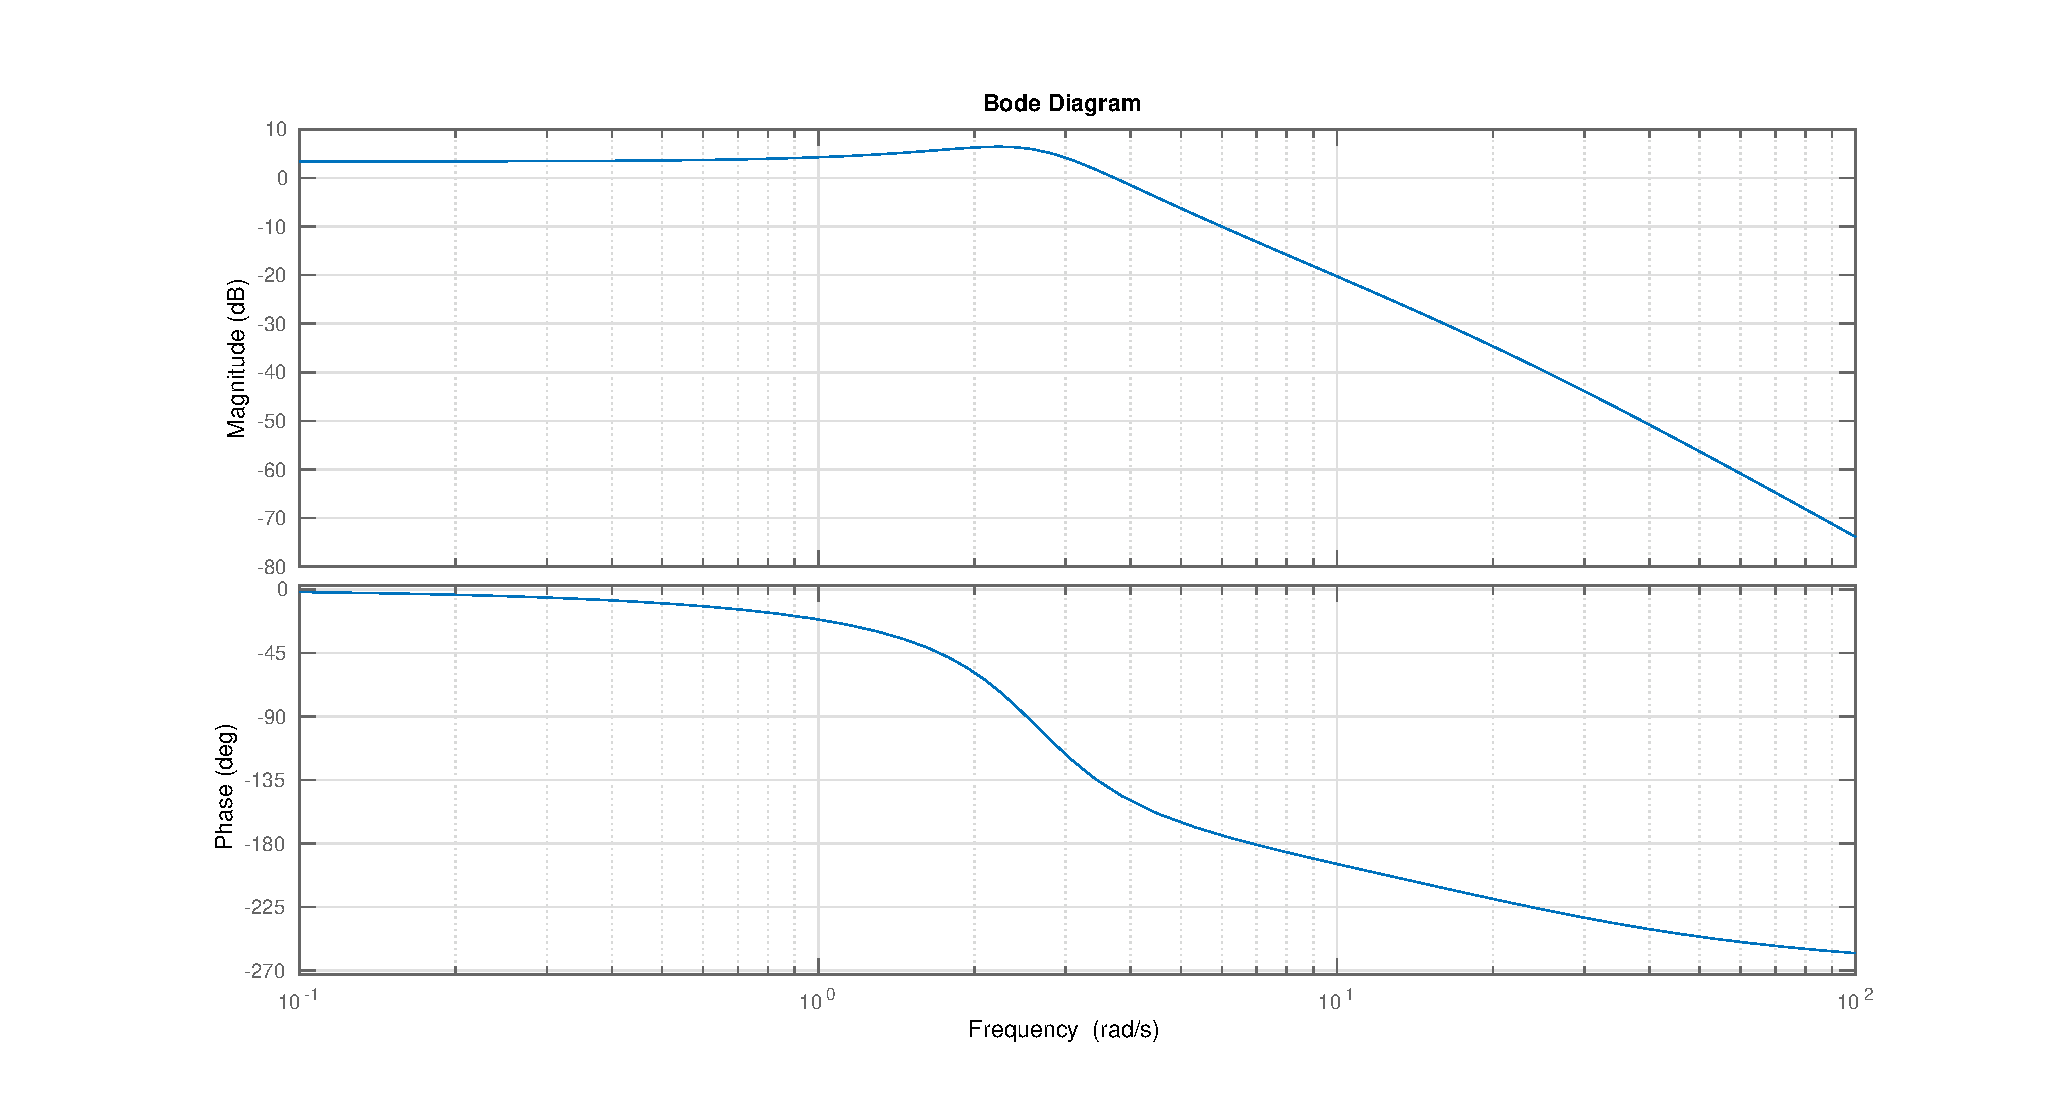
\includegraphics[width=\textwidth]{leccion-bode.eps}
\end{figure}

Con esto en mente, complete las siguientes actividades: 
\begin{enumerate}[label=\alph*.]
\item \textbf{[4 Puntos]} Calcule los m\'argenes de ganancia y fase del sistema. \\[1ex] \emph{Soluci\'on:}
\begin{itemize}
\item Para encontrar el margen de ganancia vemos que la fase es $-180\deg$ cuando \linebreak $\omega \approx 7.5$ rad/s. Para esta frecuencia la magnitud es $-15$ dB, por lo que: 
\[
G_M \; \approx \; 15 \, \text{dB}
\]
\item Para encontrar el margen de fase observamos que la magnitud es 0 dB cuando $\omega \approx 3.5$ rad/s. Para esta frecuencia la fase es $135\deg$, por lo que: 
\[
\phi_M \; \approx \; 45\deg
\]

\end{itemize}


\item Suponiendo que el sistema es puesto en un lazo de retro-alimentaci\'on unitaria, compute las siguientes m\'etricas de desempe\~no del sistema en circuito cerrado: 
\begin{itemize}
\item \textbf{[3 Puntos]} Error en estado estable para una entrada escal\'on. \\[1ex] \emph{Soluci\'on:} Reconociendo que la as\'intota de baja frecuencia se encuentra a unos tres o cuatro decibeles, tenemos: 
\[
20 \, \log_{10}( K_p ) \; \approx \; 3.5 \quad \Longrightarrow \quad
K_p \; \approx \; 1.5
\]
Consecuentemente, el error en estado estable para una entrada escal\'on es: 
\[
e_{step}(\infty) \; = \; \frac{1}{1 + K_p} \; \approx \; 0.4
\; \equiv \; 40\%
\]
\item \textbf{[3 Puntos]} Porcentage de sobrepaso. \\[1ex] \emph{Soluci\'on:} El margen de fase es de unos 45\deg lo que corresponde a una tasa de amortiguamiento $\zeta \approx 0.5$ tal como se muestra en la figura de abajo. Consecuentemente el porcentaje de sobrepaso es: 
\[
OS \; = \; \exp \left(
- \frac{ \zeta \, \pi}{ \sqrt{1 - \zeta^2}}
\right) \; \approx \; 0.163 \; \equiv \; 16.3\%
\]
\begin{figure}[htb]
\centering
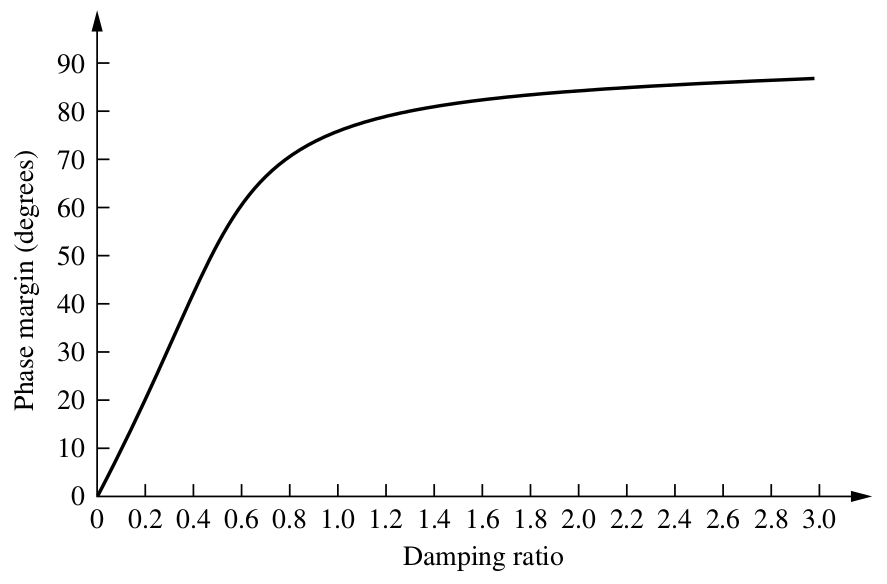
\includegraphics[width=0.72\textwidth]{Fig_phase-damping.jpg}
\end{figure}

\end{itemize}
\end{enumerate}

\end{problem}
\vspace{\baselineskip}

\end{document}
